%%
%% This is file `sample-sigplan.tex',
%% generated with the docstrip utility.
%%
%% The original source files were:
%%
%% samples.dtx  (with options: `all,proceedings,bibtex,sigplan')
%% 
%% IMPORTANT NOTICE:
%% 
%% For the copyright see the source file.
%% 
%% Any modified versions of this file must be renamed
%% with new filenames distinct from sample-sigplan.tex.
%% 
%% For distribution of the original source see the terms
%% for copying and modification in the file samples.dtx.
%% 
%% This generated file may be distributed as long as the
%% original source files, as listed above, are part of the
%% same distribution. (The sources need not necessarily be
%% in the same archive or directory.)
%%
%%
%% Commands for TeXCount
%TC:macro \cite [option:text,text]
%TC:macro \citep [option:text,text]
%TC:macro \citet [option:text,text]
%TC:envir table 0 1
%TC:envir table* 0 1
%TC:envir tabular [ignore] word
%TC:envir displaymath 0 word
%TC:envir math 0 word
%TC:envir comment 0 0
%%
%%
%% The first command in your LaTeX source must be the \documentclass
%% command.
%%
%% For submission and review of your manuscript please change the
%% command to \documentclass[manuscript, screen, review]{acmart}.
%%
%% When submitting camera ready or to TAPS, please change the command
%% to \documentclass[sigconf]{acmart} or whichever template is required
%% for your publication.
%%
%%
\documentclass[sigplan,screen]{acmart}

%%
%% \BibTeX command to typeset BibTeX logo in the docs
\AtBeginDocument{%
  \providecommand\BibTeX{{%
    Bib\TeX}}}

%% Rights management information.  This information is sent to you
%% when you complete the rights form.  These commands have SAMPLE
%% values in them; it is your responsibility as an author to replace
%% the commands and values with those provided to you when you
%% complete the rights form.
\setcopyright{acmlicensed}
\copyrightyear{2024}
\acmYear{2018}
\acmDOI{XXXXXXX.XXXXXXX}

%% These commands are for a PROCEEDINGS abstract or paper.
\acmConference[Cloud computing e infraestructura para Big Data]{Make sure to enter the correct
  conference title from your rights confirmation emai}{Agosto 31-08,
  2024}{Santa Cruz, Bolivia}
%%
%%  Uncomment \acmBooktitle if the title of the proceedings is different
%%  from ``Proceedings of ...''!
%%
%%\acmBooktitle{Woodstock '18: ACM Symposium on Neural Gaze Detection,
%%  June 03--05, 2018, Woodstock, NY}
\acmISBN{978-1-4503-XXXX-X/18/06}


%%
%% Submission ID.
%% Use this when submitting an article to a sponsored event. You'll
%% receive a unique submission ID from the organizers
%% of the event, and this ID should be used as the parameter to this command.
%%\acmSubmissionID{123-A56-BU3}

%%
%% For managing citations, it is recommended to use bibliography
%% files in BibTeX format.
%%
%% You can then either use BibTeX with the ACM-Reference-Format style,
%% or BibLaTeX with the acmnumeric or acmauthoryear sytles, that include
%% support for advanced citation of software artefact from the
%% biblatex-software package, also separately available on CTAN.
%%
%% Look at the sample-*-biblatex.tex files for templates showcasing
%% the biblatex styles.
%%

%%
%% The majority of ACM publications use numbered citations and
%% references.  The command \citestyle{authoryear} switches to the
%% "author year" style.
%%
%% If you are preparing content for an event
%% sponsored by ACM SIGGRAPH, you must use the "author year" style of
%% citations and references.
%% Uncommenting
%% the next command will enable that style.
%%\citestyle{acmauthoryear}
\usepackage{tabularx}
\usepackage{graphicx}
\usepackage[spanish]{babel}

\newcommand{\staricon}[1]{
    \begin{tikzpicture}[scale=#1]
        \filldraw[fill=yellow, draw=black] 
        (0,0) -- (0.2,0.6) -- (0.6,0.6) -- (0.3,0.9) -- (0.4,1.4) -- (0,1.1) -- (-0.4,1.4) -- (-0.3,0.9) -- (-0.6,0.6) -- (-0.2,0.6) -- cycle;
    \end{tikzpicture}
}

%%
%% end of the preamble, start of the body of the document source.
\begin{document}

%%
%% The "title" command has an optional parameter,
%% allowing the author to define a "short title" to be used in page headers.
\title{Visualizers: Athena vs. Looker Studio}

%%
%% The "author" command and its associated commands are used to define
%% the authors and their affiliations.
%% Of note is the shared affiliation of the first two authors, and the
%% "authornote" and "authornotemark" commands
%% used to denote shared contribution to the research.
\author{Bravo Peña}
\author{Darlyn}
\affiliation{
  \institution{UAGRM}
  \city{Santa Cruz}
  \country{Bolivia}
}
\email{contact@bpdarlyn.com}

\author{Torrejón Mendez}
\author{Joel Gabriel}
\affiliation{
  \institution{UAGRM}
  \city{Santa Cruz}
  \country{Bolivia}
}
\email{joel.torrejon.mendez@gmail.com}

\author{Valle Tamayo}
\author{Brandon Jason}
\affiliation{
  \institution{UAGRM}
  \city{Santa Cruz}
  \country{Bolivia}}
\email{bjvtamayo78@gmail.com}
%%
%% By default, the full list of authors will be used in the page
%% headers. Often, this list is too long, and will overlap
%% other information printed in the page headers. This command allows
%% the author to define a more concise list
%% of authors' names for this purpose.
\renewcommand{\shortauthors}{Bravo - Torrejón - Valle}

%%
%% The code below is generated by the tool at http://dl.acm.org/ccs.cfm.
%% Please copy and paste the code instead of the example below.
%%
% \begin{CCSXML}
% <ccs2012>
%  <concept>
%   <concept_id>00000000.0000000.0000000</concept_id>
%   <concept_desc>Do Not Use This Code, Generate the Correct Terms for Your Paper</concept_desc>
%   <concept_significance>500</concept_significance>
%  </concept>
%  <concept>
%   <concept_id>00000000.00000000.00000000</concept_id>
%   <concept_desc>Do Not Use This Code, Generate the Correct Terms for Your Paper</concept_desc>
%   <concept_significance>300</concept_significance>
%  </concept>
%  <concept>
%   <concept_id>00000000.00000000.00000000</concept_id>
%   <concept_desc>Do Not Use This Code, Generate the Correct Terms for Your Paper</concept_desc>
%   <concept_significance>100</concept_significance>
%  </concept>
%  <concept>
%   <concept_id>00000000.00000000.00000000</concept_id>
%   <concept_desc>Do Not Use This Code, Generate the Correct Terms for Your Paper</concept_desc>
%   <concept_significance>100</concept_significance>
%  </concept>
% </ccs2012>
% \end{CCSXML}

% \ccsdesc[500]{Do Not Use This Code~Generate the Correct Terms for Your Paper}
% \ccsdesc[300]{Do Not Use This Code~Generate the Correct Terms for Your Paper}
% \ccsdesc{Do Not Use This Code~Generate the Correct Terms for Your Paper}
% \ccsdesc[100]{Do Not Use This Code~Generate the Correct Terms for Your Paper}

%%
%% Keywords. The author(s) should pick words that accurately describe
%% the work being presented. Separate the keywords with commas.
% \keywords{Do, Not, Us, This, Code, Put, the, Correct, Terms, for,
%   Your, Paper}
%% A "teaser" image appears between the author and affiliation
%% information and the body of the document, and typically spans the
%% page.
\begin{teaserfigure}
  
\includegraphics[width=\textwidth]{images/logo_soe.png}
  \Description{Enjoying the baseball game from the third-base
  seats. Ichiro Suzuki preparing to bat.}
  \label{fig:teaser}
\end{teaserfigure}

\received{20 February 2007}
\received[revised]{12 March 2009}
\received[accepted]{5 June 2009}

%%
%% This command processes the author and affiliation and title
%% information and builds the first part of the formatted document.
\maketitle

% Document content
\section{Introducción}
ACM's consolidated article template, introduced in 2017, provides a
consistent \LaTeX\ style for use across ACM publications, and
incorporates accessibility and metadata-extraction functionality
necessary for future Digital Library endeavors. Numerous ACM and
SIG-specific \LaTeX\ templates have been examined, and their unique
features\cite{ibm-sl} incorporated into this single new template.

If you are new to publishing with ACM, this document is a valuable
guide to the process of preparing your work for publication. If you
have published with ACM before, this document provides insight and
instruction into more \cite{ibm-ml} recent changes to the article template.

The ``\verb|acmart|'' document class can be used to prepare articles
for any ACM publication --- conference or journal, and for any stage
of publication, from\cite{ibm-usl} review to final ``camera-ready'' copy, to the
author's own version, with {\itshape very} few changes to the source.

\section{Data Visualization}
La visualización de datos es la representación de datos mediante el
uso de gráficos comunes, como diagramas, gráficos, infografías e 
incluso animaciones. Estas presentaciones visuales de información
comunican relaciones complejas entre datos y perspectivas basadas
en datos de una manera fácil de entender. \cite{ibm-data-visualization}


\subsection{Importancia}
Las empresas modernas suelen procesar grandes volúmenes de datos
procedentes de diversas fuentes, como las siguientes:

\begin{itemize}
  \item {\textbf{Sitios web internos y externos}}
  \item {\textbf{Dispositivos inteligentes}}
  \item {\textbf{Redes sociales}}
  \item {\textbf{Sistemas internos de recopilación de datos}}
\end{itemize}

Sin embargo, los datos sin procesar pueden ser difíciles de
comprender y utilizar. Por ello, los científicos de datos preparan
y presentan los datos en el contexto adecuado. Les dan una forma
visual para que los responsables de la toma de decisiones puedan
identificar las relaciones entre los datos y detectar patrones o
tendencias ocultas. La visualización de datos crea historias que
hacen avanzar la inteligencia empresarial y respaldan la toma de
decisiones basada en datos y la planificación estratégica.

\subsection{Beneficios}
Algunos beneficios de la visualización de datos son los siguientes:

\begin{itemize}
  \item {\textbf{Toma de decisiones estratégicas :}} Las partes interesadas
  clave y la alta dirección utilizan la visualización de datos para interpretarlos
  de forma significativa. Ahorran tiempo gracias a un análisis de datos más
  rápido y a la capacidad de visualizar el panorama general. Por ejemplo,
  pueden identificar patrones, descubrir tendencias y obtener información
  para mantenerse por delante de la competencia.
  \item {\textbf{Servicio al cliente mejorado :}} La visualización de datos
  resalta las necesidades y deseos de los clientes mediante una representación
  gráfica. Puede identificar deficiencias en su servicio al cliente, mejorar
  estratégicamente los productos o servicios y reducir las ineficiencias operativas.
  \item {\textbf{Mayor compromiso de los empleados :}} Las técnicas de visualización
  de datos son útiles para comunicar los resultados del análisis de datos a un
  equipo grande. Todo el grupo puede visualizar los datos en conjunto para
  desarrollar objetivos y planes comunes. Pueden utilizar el análisis visual para medir
  los objetivos y el progreso y mejorar la motivación del equipo. Por ejemplo, un
  equipo de ventas trabaja en conjunto para aumentar la altura de su gráfico de barras
  de ventas en un trimestre.
\end{itemize}

\subsection{Mejores prácticas}
Con tantas herramientas de visualización de datos disponibles, también ha aumentado
la visualización de información ineficaz. La comunicación visual debe ser simple
y deliberada para garantizar que la visualización de datos ayude a su público
objetivo a llegar a la información o conclusión deseada. Las siguientes prácticas
recomendadas pueden ayudar a garantizar que la visualización de datos sea útil
y clara:

\begin{itemize}
  \item {\textbf{Conozca a su audiencia :}} Piense para quién está diseñada su
  visualización y luego asegúrese de que la visualización de datos se ajuste a
  sus necesidades.
  \item {\textbf{Elija un elemento visual eficaz :}} Existen elementos visuales
  específicos diseñados para tipos específicos de conjuntos de datos. Por ejemplo,
  los diagramas de dispersión muestran bien la relación entre dos variables,
  mientras que los gráficos de líneas muestran bien los datos de series temporales.
  Asegúrese de que el elemento visual realmente ayude a la audiencia a comprender
  la idea principal.
  \item {\textbf{Manténgalo simple :}} Las herramientas de visualización de datos
  pueden facilitar la incorporación de todo tipo de información a su elemento visual.
  Sin embargo, el hecho de que pueda hacerlo no significa que deba hacerlo. En la
  visualización de datos, debe ser muy deliberado con respecto a la información
  adicional que agrega para centrar la atención del usuario.
\end{itemize}
\section{Kong}
As noted in the introduction, the ``\verb|acmart|'' document class can
be used to prepare many different kinds of documentation --- a
double-anonymous initial submission of a full-length technical paper, a
two-page SIGGRAPH Emerging Technologies abstract, a ``camera-ready''
journal article, a SIGCHI Extended Abstract, and more --- all by
selecting the appropriate {\itshape template style} and {\itshape
  template parameters}.

This document will explain the major features of the document
class. For further information, the {\itshape \LaTeX\ User's Guide} is
available from
\url{https://www.acm.org/publications/proceedings-template}.

\subsection{Template Styles}

The primary parameter given to the ``\verb|acmart|'' document class is
the {\itshape template style} which corresponds to the kind of publication
or SIG publishing the work. This parameter is enclosed in square
brackets and is a part of the {\verb|documentclass|} command:
\begin{verbatim}
  \documentclass[STYLE]{acmart}
\end{verbatim}

Journals use one of three template styles. All but three ACM journals
use the {\verb|acmsmall|} template style:
\begin{itemize}
\item {\texttt{acmsmall}}: The default journal template style.
\item {\texttt{acmlarge}}: Used by JOCCH and TAP.
\item {\texttt{acmtog}}: Used by TOG.
\end{itemize}

The majority of conference proceedings documentation will use the {\verb|acmconf|} template style.
\begin{itemize}
\item {\texttt{sigconf}}: The default proceedings template style.
\item{\texttt{sigchi}}: Used for SIGCHI conference articles.
\item{\texttt{sigplan}}: Used for SIGPLAN conference articles.
\end{itemize}

\subsection{Template Parameters}

In addition to specifying the {\itshape template style} to be used in
formatting your work, there are a number of {\itshape template parameters}
which modify some part of the applied template style. A complete list
of these parameters can be found in the {\itshape \LaTeX\ User's Guide.}

Frequently-used parameters, or combinations of parameters, include:
\begin{itemize}
\item {\texttt{anonymous,review}}: Suitable for a ``double-anonymous''
  conference submission. Anonymizes the work and includes line
  numbers. Use with the \texttt{\acmSubmissionID} command to print the
  submission's unique ID on each page of the work.
\item{\texttt{authorversion}}: Produces a version of the work suitable
  for posting by the author.
\item{\texttt{screen}}: Produces colored hyperlinks.
\end{itemize}

This document uses the following string as the first command in the
source file:
\begin{verbatim}
\documentclass[sigplan,screen]{acmart}
\end{verbatim}

\section{Amazon API Gateway}

Amazon API Gateway \cite{aws-api-gateway-docs} es un servicio que ofrece claves fundamentales que todo API Gateway debería tener: \
\begin{itemize}
	\item Único punto de entrada
	\item Conductor de Rutas
	\item Protocolo de transformación
	\item Registry and Discovery
	\item Autenticación y Autorización
	\item Escalabilidad y Orquestación
	\item Thortting (Limites)
	\item Monitorización
\end{itemize}

Pero tiene características adicionales como : \

\begin{itemize}
	\item Son basadas en HTTP
	\item Son basadas en websockets
	\item Forma parte de un set de infraestructura llamada serverless (pay as you go)
\end{itemize}
\subsection{Arquitectura}
\begin{figure}[htbp]
	\centering
	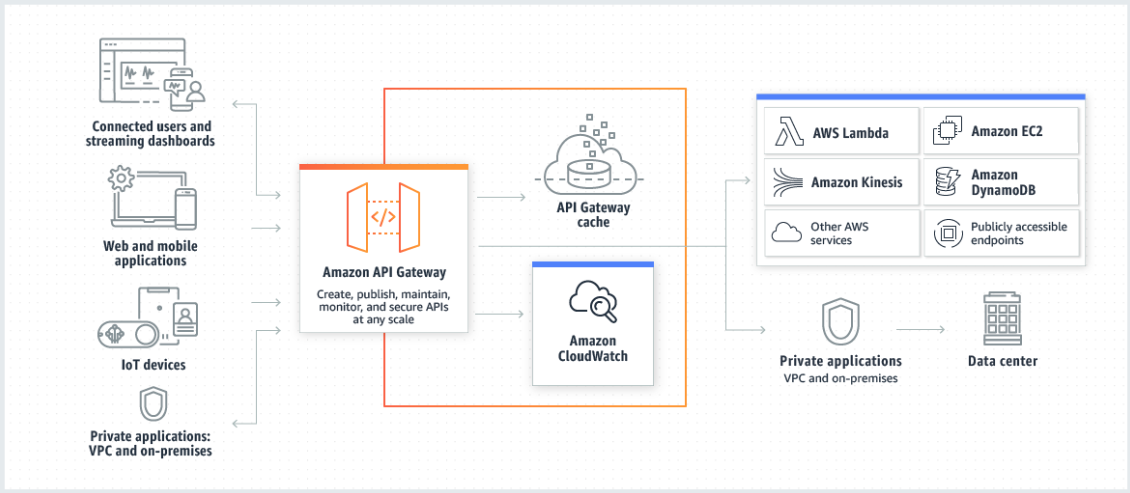
\includegraphics[width=\columnwidth]{images/architecture_aws_api_gateway}
	\caption{Arquitectura general de Aws API Gateway}
	\label{fig:architecture_aws_api_gateway}
\end{figure}

\subsection{Autenticación}
A pesar de ser un servicio de paga su autenticación es muy flexible porque te permite usar un proveedor existente de AWS tales como: AWS Identity, Access Management policies, Lambda authorizer y Amazon Cognito

\subsection{Tipos de Endpoints}
Amazon ofrece 2 tipos de Endpoints más usados:
\subsubsection{Edge Optimized API endpoints}
Las solicitudes se enrutan al Cloudfront más cercano, Point of Presence(POP). El cuál ayuda si tus clientes están distribuídos geográficamente, cuando creas un API Gateway y mantienes muchos de los parámetros por defecto no necesitas configurar esta opción ya que es el comportamiento predeterminado.

\subsubsection{Tipo de Endpoint Regional}
Especial para clientes en la misma región, por ejemplo cuando algún cliente que tiene una instancia de EC2 llama una api que también se encuentra en la misma región o también cuando necesitas baja latencia o respuesta rápida, al limitar la comunicación dentro de una región se minimiza las latencias y los costos asociados a la red.

\subsection{Integraciones}
Una vez que se define un API Method (POST, PUT, DELETE, ETC) tu necesitas definir un backend endpoint que puede ser cualquiera de:\
\begin{itemize}
	\item Ejecutar un Service Action como: SQS, STEPFUNCTION
	\item Función \textbf{Lambda}
	\item Otro \textbf{HTTP Endpoint}
\end{itemize}

Para la comunicación con el backend tu necesitas definir: \

\begin{description}
	\item[Integration Request:] Como quieres formatear la solicitud para posteriormente enviar la request formateada a tu backend
	\item[Integration Response:] Cómo quieres formatear la respuesta del backend para ser respondida al client.
\end{description}

\subsection{Validaciones}
Puedes definir validaciones antes de ejecutar tu backend, reduciendo ejecuciones innecesarias en tu backend, ya que api gateway puede retornar un error 400 al cliente sin pasar por el backend.

\subsection{Transformaciones de Data}
Te permite trasformar tu data, usando un motor de expresiones tu puedes cambiar, los headers, query arguments, body usando \textbf{mapping templates}.

\subsection{OpenApi}
Si ya tenías o usas OpenApi para definir tus endpoints puedes continuar haciendolo y agregar algunos campos adicionales para desplegar estos endpoints en API Gateway sin necesidad de definirlos de forma manual o usando IAAC.
De momento solo ofrece soporte para \textbf{OpenApi v2.0} y \textbf{OpenApi v3.0}
\subsection{Seguridad}
puedes configurar solicitudes cruzadas por endpoint (api method). También debido a que AWS tiene habilitado de forma predeterminada la detección de ataques de RED como un DOS estas siendo protegido también por toda la estructura de AWS.

\subsection{Compartir Endpoints a tus Clientes}
Puedes configurar API Keys para tus clientes y también puedes configurar También definir cuotas por API que tus clientes pueden usar así como el throttling que tus customers deben tener y si sobre pasa de estos límites Api Gateway rechazará automáticamente la solicitud.

\subsection{Monitorización}
Tienes innumerables métricas diseñadas por AWS, puedes también hacer uso de Cloudwatch logs y X-Ray. Además que en los mismos servicios puedes subscribirte a métricas y recibiendo alarmas de los eventos que 
\section{Looker Studio}
\section{Benchmark}

\begin{table}[h!]
\centering
\caption{Comparación entre Power BI, AWS QuickSight y Looker Studio}
\renewcommand{\arraystretch}{1.5} % Aumenta el espacio entre filas
\setlength{\tabcolsep}{5pt} % Aumenta el espacio entre columnas
\begin{tabular}{|l|c|c|c|c|}
\hline
\textbf{Característica} & \textbf{Power BI} & \textbf{AWS QuickSight} & \textbf{Looker Studio} & \textbf{Ganador} \\ \hline
\textbf{Integración con ecosistemas} & Sí & Sí & Sí & Todas \\ \hline
\textbf{Interfaz de usuario} & Sí & Sí & Sí & Looker Studio \\ \hline
\textbf{Manipulación de datos} & Sí & Sí & Sí & Power BI \\ \hline
\textbf{Análisis de datos en tiempo real} & Sí & Sí & Sí & Looker Studio \\ \hline
\textbf{Visualización de datos} & Sí & Sí & Sí & Looker Studio \\ \hline
\textbf{Colaboración} & Sí & Sí & Sí & Power BI \\ \hline
\textbf{Integración de datos} & Sí & Sí & Sí & Power BI \\ \hline
\textbf{Modelado de datos} & Sí & Sí & No & Power BI \\ \hline
\textbf{Precio} & No & Sí & Sí & Looker Studio / AWS QuickSight \\ \hline
\textbf{Comunidad y soporte} & Sí & Sí & No & Power BI \\ \hline
\end{tabular}
\end{table}
    
\section{Conclusión}

Existe una fuerte competencia entre Looker Studio, Power BI, y AWS QuickSight. 
Las tres herramientas destacan en diferentes aspectos de la inteligencia empresarial.

Y podemos decir: 
\begin{itemize}
  \item \textbf{Power BI.} Si el usuario se siente comodo como capacidades avanzadas y se puede justificar el costo ya que Power BI ofrece una manipulación de datos robusta, modelado de datos avanzado, y una comunidad de soporte extensa.
  \item \textbf{Looker Studio.} Ideal para usuarios profundamente integrados en el ecosistema de Google, ofreciendo una interfaz simple y fuertes capacidades de análisis en tiempo real.
  \item \textbf{AWS QuickSight.} Una opción sólida para aquellos en el ecosistema de AWS, proporcionando una fuerte integración y capacidades en tiempo real a un precio competitivo.
\end{itemize}
No hay mejores que otras simplemente la diferencia estará en las capacidades que tiene el usuario de conocer la herramienta y de como enfrenta el problema.


%%
%% The acknowledgments section is defined using the "acks" environment
%% (and NOT an unnumbered section). This ensures the proper
%% identification of the section in the article metadata, and the
%% consistent spelling of the heading.
% \begin{acks}
% To Robert, for the bagels and explaining CMYK and color spaces.
% \end{acks}

%%
%% The next two lines define the bibliography style to be used, and
%% the bibliography file.
\bibliographystyle{ACM-Reference-Format}
\bibliography{bibliography}


%%
%% If your work has an appendix, this is the place to put it.
\appendix

\end{document}
\endinput
%%
%% End of file `sample-sigplan.tex'.